\documentclass[11pt]{article}
\usepackage[a4paper, portrait, margin=1in]{geometry}
\usepackage{hyperref}

\usepackage{graphicx}
% Fancy header package for version number

\usepackage{fancyhdr}
\pagestyle{fancy}
\fancyhf{}
\renewcommand{\headrulewidth}{0pt}
\renewcommand{\footrulewidth}{0pt}

\fancypagestyle{firstpagefooter}
{
\lfoot{Version: 29.09.2016}
\cfoot{}
\rfoot{\thepage}
}
\cfoot{\thepage}

\begin{document}

\title{Advanced Systems Lab (Fall'16) -- First
Milestone}

\author{\textbf{Name: \emph{Jinank Jain}}\\\textbf{Legi number: \emph{16-932-881}}}

\date{
\vspace{4cm}
\textbf{Grading} \\
\begin{tabular}{|c|c|}
\hline  \textbf{Section} & \textbf{Points} \\
\hline  1.1 &  \\ 
\hline  1.2 &  \\ 
\hline  1.3 &  \\ 
\hline  1.4 &  \\ 
\hline  2.1 &  \\ 
\hline  2.2 &  \\ 
\hline  3.1 &  \\ 
\hline  3.2 &  \\ 
\hline  3.3 &  \\ 
\hline \hline Total & \\
\hline 
\end{tabular} 
}

\maketitle
\thispagestyle{firstpagefooter}
\newpage

\section{System Description}\label{sec:system-description}

\subsection{Overall Architecture}\label{sec:desc:architecture}

\begin{figure}[h]
    \centering
    \includegraphics[width=0.8\textwidth]{class.png}
    \caption{Class Diagram}
    \label{fig:class}
\end{figure}

\begin{figure}[h]
    \centering
    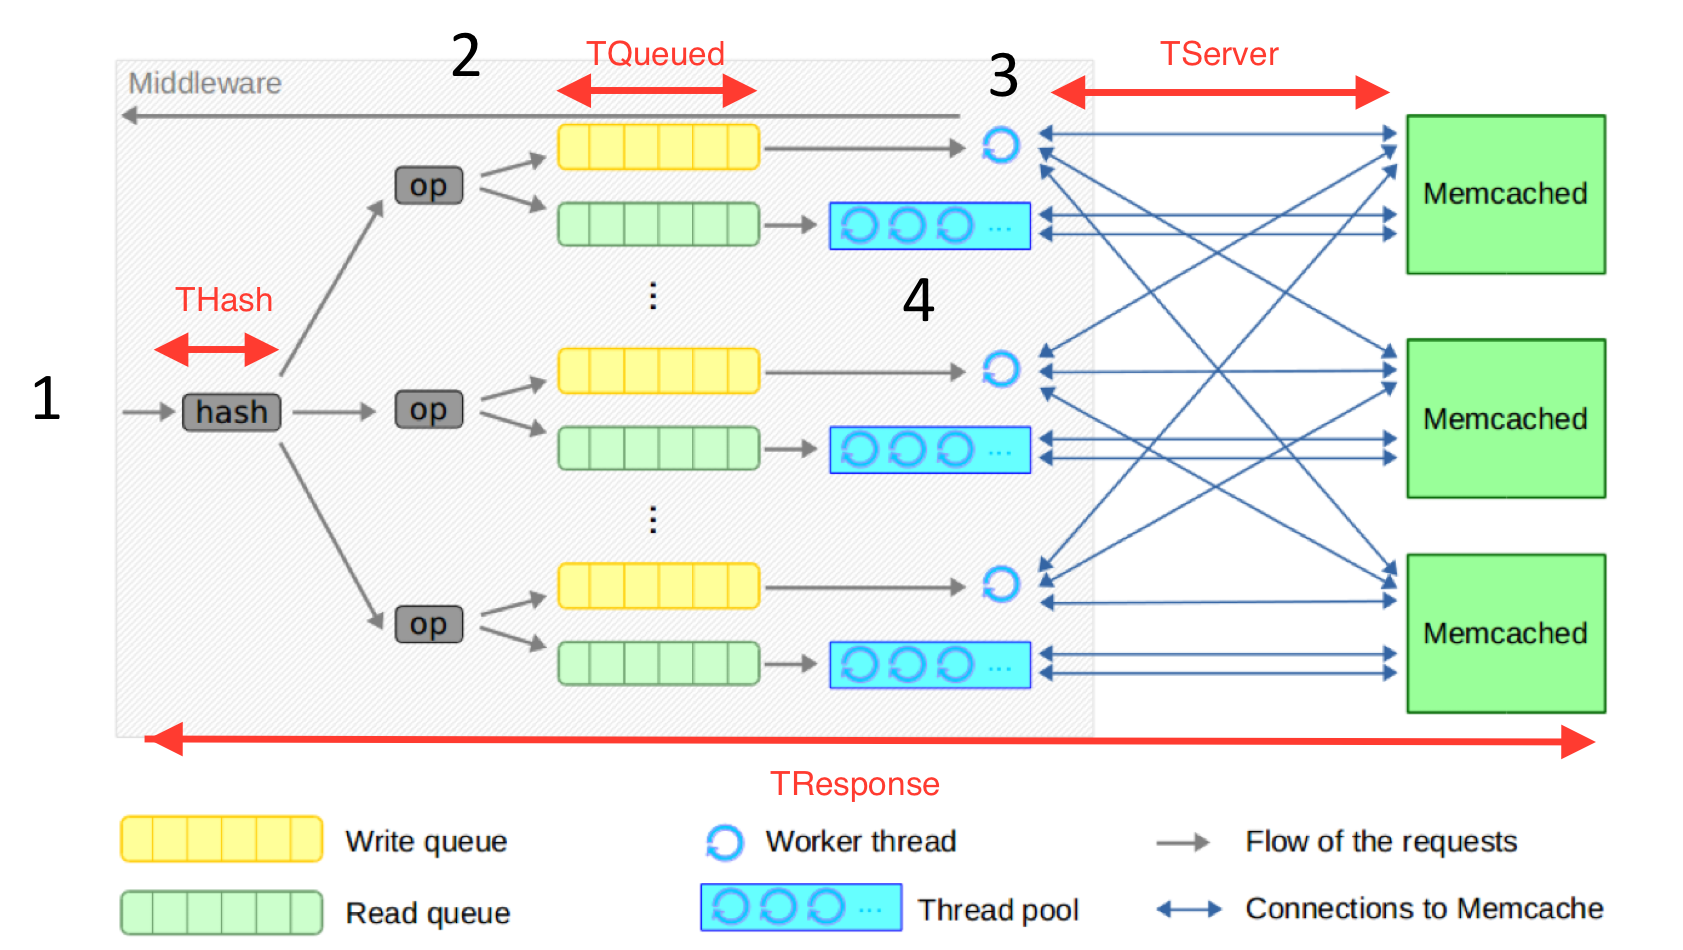
\includegraphics[width=0.9\textwidth]{des.png}
    \caption{Project Description}
    \label{fig:des}
\end{figure}

In an abstract way Figure \ref{fig:class} explains the complete system architecture. The whole project is kind of divided into 4 parts as show in Figure \ref{fig:des}. RunMW.java which was a wrapper provided to us creates an instance of NioServer which accepts connection from memaslap and start reading content from socket channel into a read buffer using Java NIO Socket Channels and Byte Buffer. One thing that is to be noted, since memaslap does not close these socket connection and keep sending data on the same socket connection so to maximize the performance I kept those connection open otherwise accepting a TCP requires a three way handshake that can cost a lot time. For reusing these socket channels I register these socket to a selector which keeps tracks of which channel is free to accept new connection and read data in their respective buffers. This all about section 1 on Figure \ref{fig:des} which is implemented in \footnote{\url{https://gitlab.inf.ethz.ch/jjain/asl-fall16-project/blob/master/middleware/src/main/middleware/NioServer.java}} 

After reading the data in the read buffer I call a function called processData() which parses the request and try to identify whether it is a GET/SET /DELETE request by looking at the first byte of the data in the read buffer and after that I parse the key into Java String and then hash it to find which server I need to send that request. After finding the appropriate server number and type of request I add into their respective queues i.e. read or write queues. One design decision which I took was treat delete as set requests and thus I add delete request into write queues and justification for this would be in delete request we are trying to call set on that key to null(i.e. empty). This all about section 2 on  Figure \ref{fig:des} which is implemented in \footnote{\url{https://gitlab.inf.ethz.ch/jjain/asl-fall16-project/blob/master/middleware/src/main/middleware/EchoWorker.java}}

\begin{itemize}
	\item $T_{response}$: Time when some socket channel starts reading content into a read buffer.
	\item $T_{queued}$: Amount of time spend in read/write queues.
	\item $T_{server}$: Time taken by memcached to send response to a particular request.
	\item $T_{hash}$ Time taken by hash function.
\end{itemize}

These timing relating things are instrumented in data structure called Load which is in the file.
\footnote{\url{https://gitlab.inf.ethz.ch/jjain/asl-fall16-project/blob/master/middleware/src/main/middleware/Load.java}}

\subsection{Load Balancing and Hashing}\label{sec:desc:hashing}

\begin{figure}[h]
    \centering
    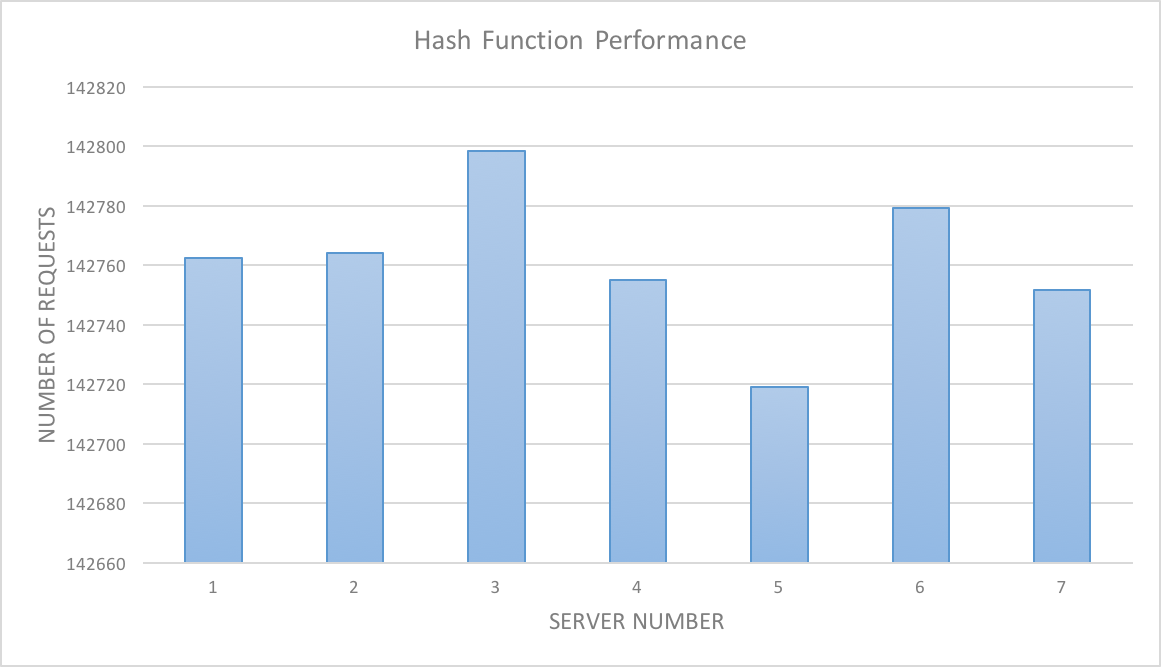
\includegraphics[width=0.6\textwidth]{hash.png}
    \caption{Hash Function Performance}
    \label{fig:hash}
\end{figure}

\textbf{\\ Goals for Hash Function:}

Since we are trying to build a load balancer, so in that case a good load balancer should distribute the load uniformly among different servers. From this the requirements of hash function are pretty clear it should distribute the key space uniformly between different servers.
\\ \\
\textbf{Hash Function Description: } 

For hashing I am using Java inbuilt hash code. If we look at the documentation of java.lang.String class implements its hashCode() using a product sum algorithm over the entire text of the string. An instance $s$ of the java.lang.String class, for example, would have a hash code $h(s)$ defined by

$$h(s) = \sum_{i=0}^{n-1} s[i]. 31^{n-1-i} $$

where terms are summed using Java 32-bit int addition, $s[i]$ $i^{th}$ character of the string, and  $n$ is the length of $s$. After calculating the hash of key I take modulo with total number of servers.
\\ \\
\textbf{Experiments with hash function}

I ran few test with the hash function as described above. As a test case I assumed that let there be 7 servers and I want to distribute some randomly generated 16 bytes keys (about 1000000 keys) on these 7 servers. I repeated this experiment for 100 times and took the average of numbers of requests that a server would receive and drawn the histogram as shown in  Figure \ref{fig:hash}. Looking at histogram we can comment that keys are distributed in a uniform fashion and maximum difference between highest and lowest request that a server receives is 79 which is pretty much acceptable. Thus choosing \textbf{hashCode()} is pretty much justified. I have included the script which I ran for performing this test \footnote{\url{https://gitlab.inf.ethz.ch/jjain/asl-fall16-project/blob/master/middleware/analytics/Hash.java}}

\subsection{Write Operations and Replication}\label{sec:desc:writes}

\textbf{Implementation:}

Write Operations and replications are implemented using single thread and collection of JAVA Nio Socket Channels which are equal to number of replication we want to perform. These socket channels are connected to respective memcached servers. So there is a 1:1 correspondence between socket channels and memcached servers and this property is being exploited via creating a HashMap from socket channel to memcached servers which is further used for identifying which memcached server is sending response and help in keeping track of how many times we have received response for a particular key.  

In order to keep track that I have received response from all the replication servers what I did was created a HashMap which maps keys (i.e. keys which are present in request) to the count, how many times we have received response for that key and if that is equal to the number of replication we want to perform I pop that key from the hash map and send response to the server. Here things become bit tricky i.e. how to identify which client we need send response. To solve this problem I have created some replication queues which is equal to number of replication we have to perform. These queues store the request which is popped out of the write queues. Since memcached servers are single threaded so responses would always maintain an order i.e. request which are sent first will get a response and thus they will always correspond to what is there at head of the Replication Queues. Through this implementation I am able to achieve complete asynchronous behavior because I don't wait for memcached to response and whenever memcached is ready with response I deliver it to respective memaslap clients. This is done with JAVA selector which I register over replication socket channel for read operation. The code corresponding to this can be found in \footnote{\url{https://gitlab.inf.ethz.ch/jjain/asl-fall16-project/blob/master/middleware/src/main/middleware/WriteQueue.java}}
\\ \\
\textbf{Difference between replication case and write one scenario:}

Difference between replication and write one scenario are following:
\begin{itemize}
	\item Size of my replication would reduce to one as compared to replication case where I would have replication queue size equal to number of replication.
	\item In case of replication HashMaps which stores number of response corresponding to particular request and check whether I had received response from all the replication server would now just check whether it had received response from original server.
\end{itemize}
\textbf{Estimation of latencies:}
\\
Parameters which would influence the latencies are following:
\begin{itemize}
	\item \textbf{Network Latency:} This would be one of the important factor in latency calculation because over the cloud network traffic is pretty hard to predict and in our case we are passing a lot of packets back and forth and thus it would be one of the major factor in estimation of latencies.
	\item \textbf{Queueing Latency:} Since we are working in a closed system and clients would not send request untill they receive a response for a previous request and while doing replication we have to wait for all the memcached server to send response to middleware. And thus queueing latency is also one of the big factor in estimation of latencies.
\end{itemize}

\textbf{Bottleneck of write operation:}

Bottleneck of the write operations are two things:
\begin{itemize}
	\item First one is the memcached server since with time, number of keys in memcached servers would increase and thus it will take long time to response for every get/set request it received.
	\item Second one could be amount of replication that I am trying to perform since with every extra replication my hash map would grow in size which would take and thus updating and querying hash maps would no longer be O(1). 
\end{itemize}

\subsection{Read Operations and Thread Pool}\label{sec:desc:reads}

\textbf{Implementation:}

Read Operation has two main components: Thread Pool and Java LinkedBlockingQueues. For Thread Pool I am running some $n$ number of threads which are passed as a argument by RunMW.java file. Each thread in the thread pool tries to take some request from ReadQueue and if it is empty then those threads goes to sleep and whenever there is some element in ReadQueue there would be an upcall to threads in Thread Pool to wake them up and process the request. All these things are provided by Java LinkedBlockingQueues. The code corresponding to this can be found in \footnote{\url{https://gitlab.inf.ethz.ch/jjain/asl-fall16-project/blob/master/middleware/src/main/middleware/ReadQueue.java}}
\\ \\
\textbf{Thread Safety:}

\begin{figure}[h]
    \centering
    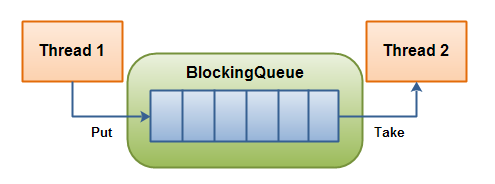
\includegraphics[scale=0.6]{blocking}
    \caption{Blocking Queues in Java}
    \label{fig:hash}
\end{figure}

For ensuring thread safety I am using Java LinkedBlockingQueue which are thread safe for implementing ReadQueue. So if we look at the implementation details in the Java Documentation for LinkedBlockingQueue it says that LinkedBlockingQueue has two locks: one on the head of the queue and other on the tail of the queue so that producer and consumer can work on that same queue without blocking each other. So when a consumer thread is trying to take an element from queue and if queue is empty that Read Thread would go to sleep and would not waste any CPU cycle and whenever there is some data in the ReadQueue there would be an upcall which would wake up those sleeping threads and start consuming from ReadQueues. Thus ensuring that this does not become the bottleneck of the system i.e. producer and consumer are able to write concurrently in the same queues.
\\ \\
\textbf{Relation between threads in the thread pool and connections to servers}

Each thread in thread pool has a socket channel which is connected to memcached server and thus there is a 1:1 to correspondence between threads in thread pool to memcached server.
\section{Memcached Baselines}\label{sec:baseline}

\textbf{Experimental Setup:}
\\
I ran the experiment with following configuration
\begin{center}
\small{
\smallskip
\begin{tabular}{|c|c|}
\hline Number of servers & 1 \\ 
\hline Number of client machines & 1 to 2 \\ 
\hline Virtual clients / machine & 1 to 64 \\ 
\hline Workload & Key 16B, Value 128B, Writes 1\% \footnotemark \\
\hline Middleware & Not present \\ 
\hline Runtime x repetitions & 30s x 5 \\ 
\hline Log files & baseline\_sample\_1.zip, baseline\_sample\_2.zip, \ldots \\
\hline 
\end{tabular} }
\end{center}

\textbf{\\Explanation of memcached behavior}
\\
Explanation about Throughput:

If we look at the graph of throughput it keeps increasing as we increase the number of clients but from the Figure \ref{fig:baset} we can say that it has a tendency to saturate as slope is decreasing with increasing number of clients. There should be an increase in throughput because with increasing number of clients memcached would be able to answer more queries which in turn will lead to increase in throughput.
\\ \\
Explanation about Average Response Time:

From normal intuition we could say that average response time should increase with increasing number of clients because with more clients we would have more request to serve and with more set request memcached server will start to slow down in sending response. That is evident from Figure \ref{fig:basea} with increasing number clients response time tends to increase which in turn increases the standard deviation for response time.
\\ \\
\textbf{Saturation Point}
\\
Looking at the Figure \ref{fig:baset} we could say that memcached has started to saturate around 128 clients and it would most probably saturate soon with some more clients.


\subsection{Throughput}\label{sec:baseline:tput}
\begin{figure}[h!]
    \centering
    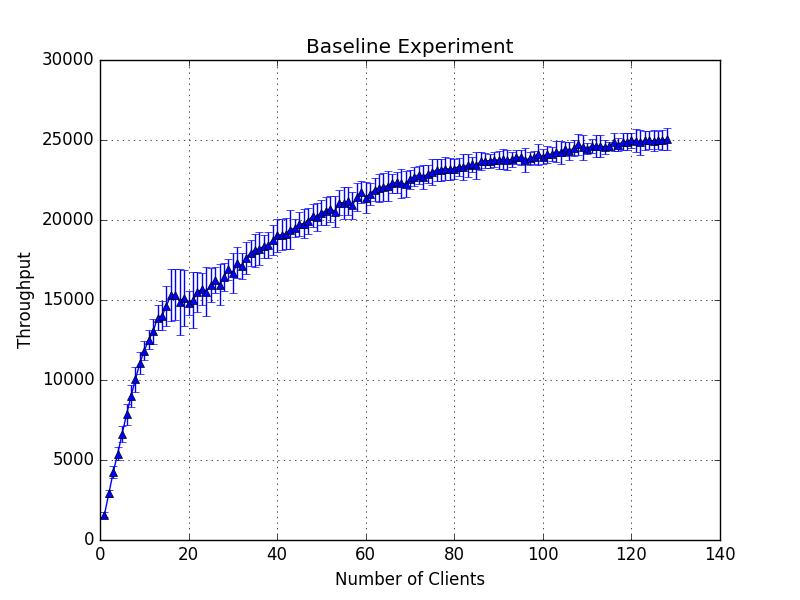
\includegraphics[width=0.7\textwidth]{base_throughput.png}
    \caption{Throughput for Baseline Experiment}
    \label{fig:baset}
\end{figure}
Some comments about Figure \ref{fig:baset}:
\begin{itemize}
	\item Throughput for 128 clients is around 25000
	\item Throughput starts to saturate around 128 clients.
	\item Standard deviation between different 5 runs is pretty low.
\end{itemize}

\subsection{Response time}\label{sec:baseline:rt}

\begin{figure}[h!]
    \centering
    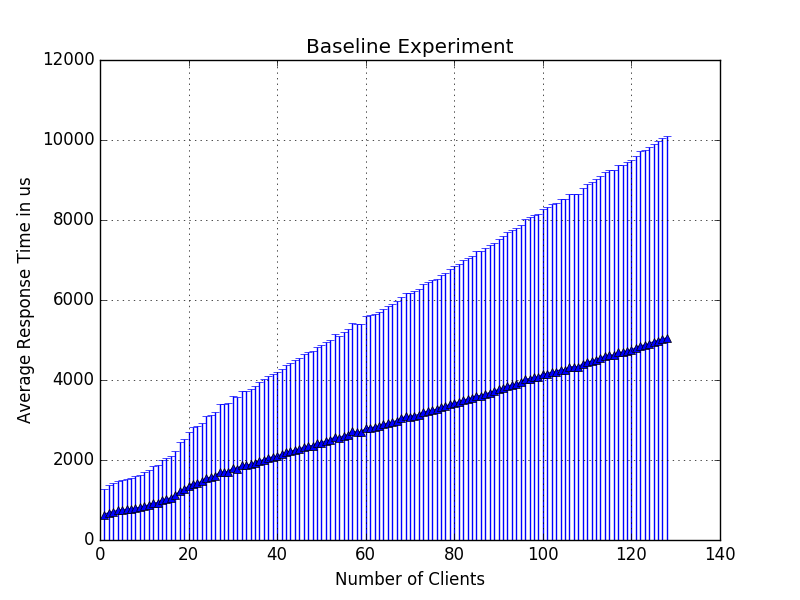
\includegraphics[width=0.7\textwidth]{base_avg.png}
    \caption{Average Response Time for Baseline Experiment}
    \label{fig:basea}
\end{figure}

Some comments about Figure \ref{fig:basea}:
\begin{itemize}
	\item Average Response time increases with increasing number of clients.
	\item Standard Deviation increases with increasing number of clients.
\end{itemize}

\section{Stability Trace}\label{sec:trace}
\textbf{Experimental Setup:}

I have run the experiment with following parameters.

\begin{center}
\small{
\smallskip
\begin{tabular}{|c|c|}
\hline Number of servers & 3 \\ 
\hline Number of client machines & 3 \\ 
\hline Virtual clients / machine &  64 \\ 
\hline Workload & Key 16B, Value 128B, Writes 1\% \\
\hline Middleware & Replicate to all (R=3) \\ 
\hline Runtime x repetitions & 1h x 1 \\ 
\hline Read Threads & 20 \\ 
\hline Log files & stablity\_client\_1.stablity\_client\_2.zip, stablity\_client\_3.zip\\
\hline 
\end{tabular} }
\end{center}



\subsection{Throughput}
\begin{figure}[h!]
    \centering
    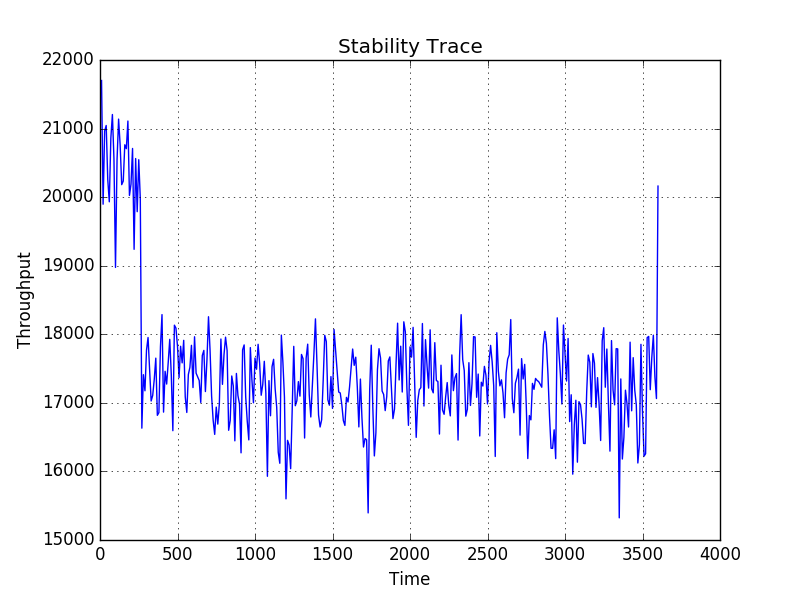
\includegraphics[width=0.7\textwidth]{stab_throughput.png}
    \caption{Throughput for Stability Trace }
    \label{fig:hash}
\end{figure}
\begin{itemize}
	\item I have some initial warmup phase since all the memaslap clients does not start at the same time since there was some delay in running them.
	\item Once all the clients come into sync phase we can notice that throughput is pretty consistent after that point.
	\item If we look at the average throughput which is around 18K.
\end{itemize}

\subsection{Response time}
\begin{figure}[h!]
    \centering
    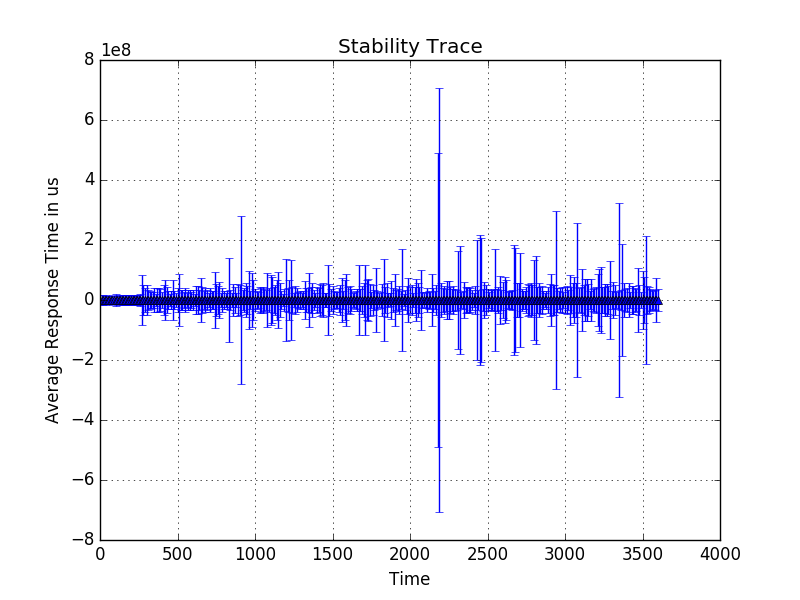
\includegraphics[width=0.7\textwidth]{stab_avg.png}
    \caption{Average Response Time for Stability Trace}
    \label{fig:hash}
\end{figure}
\footnote{For Higher resolution graphs and diagram look into this folder \url{https://gitlab.inf.ethz.ch/jjain/asl-fall16-project/blob/master/middleware/higher_res}}

\begin{itemize}
	\item If we look at average response time graph except some weird peaks which might be due to some cloud network traffic congestion and Java Garbage collector might have kicked in.
	\item Average Response time is around 7ms which is pretty good response keeping in mind we are replicating over three servers.
\end{itemize}
\subsection{Overhead of middleware}

For comparing performance we have to come on equal grounds first of all if we look at the baseline experiments we are doing those experiments with less clients and no replication. So in order to come on equal ground we have to assume some factor which is caused by extra replication. So if we look at the baseline graphs and look at the throughput for 64 clients it is around 22K and if we look at the stability trace average throughput is around 18K. Looking at this numbers we could say that replication overhead is around 20\% which is pretty much acceptable factor because of network latency and queueing latency.

And if we look at the average response time for 64 clients in baseline experiment is around 6.2 ms while if we look at the average response time from stability trace is around 7ms with much less standard deviation as compared to baseline experiment which is also pretty much acceptable because as we are performing replication and there are more clients which are sending more request which would increase average response because memcached server have more set request and they will take more time response.

\pagebreak

\section*{Logfile listing}

\begin{tabular}{|c|l|}
\hline \textbf{Short name }& \textbf{Location} \\ 
\hline microbench1 & \url{https://gitlab.inf.ethz.ch/jjain/asl-fall16-project/blob/master/baseline_sample_1.zip} \\ 
\hline microbench2 & \url{https://gitlab.inf.ethz.ch/jjain/asl-fall16-project/blob/master/baseline_sample_2.zip} \\
\hline microbench3 & \url{https://gitlab.inf.ethz.ch/jjain/asl-fall16-project/blob/master/baseline_sample_3.zip} \\
\hline microbench4 & \url{https://gitlab.inf.ethz.ch/jjain/asl-fall16-project/blob/master/baseline_sample_4.zip} \\
\hline microbench5 & \url{https://gitlab.inf.ethz.ch/jjain/asl-fall16-project/blob/master/baseline_sample_5.zip} \\
\hline trace1 & \url{https://gitlab.inf.ethz.ch/jjain/asl-fall16-project/blob/master/stablity_client_1.zip} \\ 
\hline trace1 & \url{https://gitlab.inf.ethz.ch/jjain/asl-fall16-project/blob/master/stablity_client_2.zip} \\ 
\hline trace1 & \url{https://gitlab.inf.ethz.ch/jjain/asl-fall16-project/blob/master/stablity_client_3.zip} \\ 
\hline 
\end{tabular} 

\end{document}
